\documentclass{beamer}
\usetheme{Madrid}
\usecolortheme{beaver}
\usepackage{graphicx}
\usepackage{listings}
\usepackage{xcolor}
\usepackage{multicol}
\usepackage{amsmath}
\usepackage{amssymb}
\usepackage[american]{circuitikz} 

\providecommand{\brak}[1]{\ensuremath{\left(#1\right)}}
\providecommand{\sbrak}[1]{\ensuremath{\left[#1\right]}}

\definecolor{codegreen}{rgb}{0,0.6,0}
\definecolor{codegray}{rgb}{0.5,0.5,0.5}
\definecolor{codepurple}{rgb}{0.58,0,0.82}
\definecolor{backcolour}{rgb}{0.95,0.95,0.92}

\lstdefinestyle{pythonStyle}{
    backgroundcolor=\color{backcolour},   
    commentstyle=\color{codegreen},
    keywordstyle=\color{magenta},
    numberstyle=\tiny\color{codegray},
    stringstyle=\color{codepurple},
    basicstyle=\ttfamily\tiny,
    breakatwhitespace=false,         
    breaklines=true,                 
    captionpos=b,                    
    keepspaces=true,                 
    numbers=left,                    
    numbersep=5pt,                  
    showspaces=false,                
    showstringspaces=false,
    showtabs=false,                  
    tabsize=2,
    language=Python
}
\lstset{style=pythonStyle}

\title{1.1.46}
\author{Puni Aditya - EE25BTECH11046}
\date{\today}

\begin{document}

\begin{frame}
\titlepage
\end{frame}

\begin{frame}{Question}
Consider the AC bridge shown below. $A, R, L,$ and $C$ have positive finite values. Then, $V_0 = 0$.
\begin{figure}
    \centering
    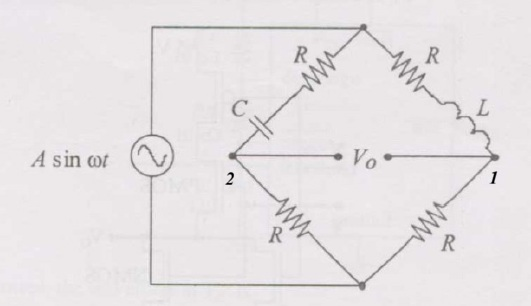
\includegraphics[width=0.3\columnwidth]{figs/circuit.jpg}
    \caption{Circuit Diagram}
	\label{fig:ckt}
\end{figure}
\begin{enumerate}
    \item $V_0 = 0$ if $\omega L = \frac{1}{\omega C}$
    \item $V_0 = 0$ if $L = C$
    \item $V_0 = 0$ if $R = \frac{1}{\omega\sqrt{LC}}$
    \item $V_0$ cannot be made zero
\end{enumerate}
\end{frame}

\begin{frame}{Theoretical Solution}
The transfer function is defined as $H(s) = \frac{V_0(s)}{V_{in}(s)}$. Applying the voltage divider rule:
\begin{align}
    V_1(s) &= V_{in}(s) \brak{\frac{R}{R + \brak{R + sL}}} = V_{in}(s) \brak{\frac{R}{2R + sL}} \\
    V_2(s) &= V_{in}(s) \brak{\frac{R}{R + \brak{R + \frac{1}{sC}}}} = V_{in}(s) \brak{\frac{sRC}{2sRC + 1}}
\end{align}
\end{frame}

\begin{frame}{Theoretical Solution}
The output voltage is $V_0(s) = V_1(s) - V_2(s)$. Thus:
\begin{align}
    H(s) &= \frac{R}{2R + sL} - \frac{sRC}{2sRC + 1} \\
    H(s) &= \frac{R\brak{2sRC + 1} - sRC\brak{2R + sL}}{\brak{2R + sL}\brak{2sRC + 1}} \\
    H(s) &= \frac{R\brak{1 - s^2LC}}{\brak{2R + sL}\brak{2sRC + 1}}
\end{align}
\end{frame}

\begin{frame}{Steady-State Analysis}
For $V_0 = 0$ in steady-state, we set $H(j\omega) = 0$:
\begin{align}
    1 - s^2LC &= 0 \implies s^2 = \frac{1}{LC}
\end{align}
Substituting $s = j\omega$ for sinusoidal steady-state:
\begin{align}
    (j\omega)^2 &= \frac{1}{LC} \\
    -\omega^2 &= \frac{1}{LC} \implies \omega^2LC = -1
\end{align}
Since $\omega, L, C > 0$, the product $\omega^2LC$ is always positive. 

\vfill
\textbf{Conclusion:} 
\textbf{(4)} No real frequency $\omega$ can satisfy $\omega^2LC = -1$. Therefore, $V_0$ cannot be zero.
\end{frame}

\begin{frame}[fragile]{Python Implementation}
\begin{lstlisting}[language=Python]
import numpy as np
from scipy import signal
import matplotlib.pyplot as plt

R, L, C = 100, 0.1, 100e-6
A, f = 10, 50
w = 2 * np.pi * f

# Transfer Function: H(s) = (R - s^2RLC) / (2s^2RLC + s(L + 4R^2C) + 2R)
num = [-R*L*C, 0, R]
den = [2*L*R*C, L + 4*R**2*C, 2*R]
sys = signal.TransferFunction(num, den)

t = np.linspace(0, 0.2, 200)
vin = A * np.sin(w * t)

tout, v0, _ = signal.lsim(sys, vin, t)

plt.plot(t, vin, label='Vin(t)', alpha=0.5, linestyle='--')
plt.plot(t, v0, label='V0(t)', linewidth=2)
plt.axhline(0, color='black', linewidth=2)
plt.axvline(0, color='black', linewidth=2)
plt.title('Time Domain Analysis of AC Bridge')
plt.xlabel('Time (s)')
plt.ylabel('Voltage (V)')
plt.legend()
plt.grid(True)
plt.savefig('plot.jpg')
plt.show()
\end{lstlisting}
\end{frame}

\begin{frame}{Simulation Results}
\begin{figure}
    \centering
    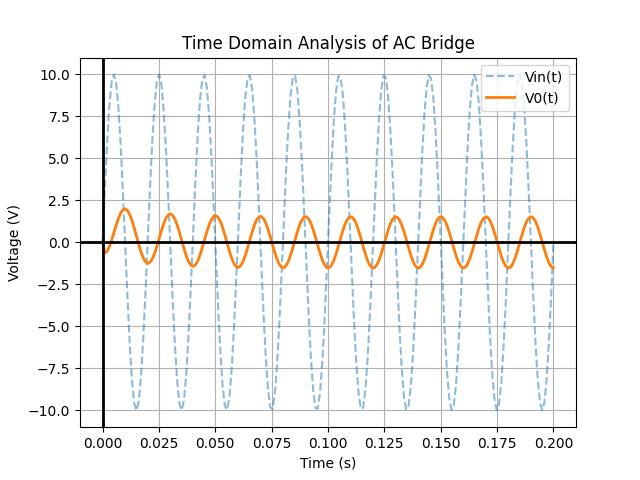
\includegraphics[width=0.5\columnwidth]{figs/plot.jpg}
    \caption{Time-Domain Response of $V_{in}$ and $V_0$}
	\label{fig:sim}
\end{figure}
The simulation confirms that $V_0(t)$ is a persistent sinusoid, meaning it never reaches a zero-amplitude steady state.
\end{frame}

\end{document}